\section{Aspectos metodologicos}
\subsection{Tipo de estudio}
El tipo de estudio identificado para el proyecto es el Descriptivo, debido a que el problema se centra en mejorar un proceso existente de administración de plataformas, el cual es repetitivo, y se desea obtener la manera de centralizar los procesos.
\subsection{Método de investigación}
	Para poder llegar al conocimiento deseado sobre el problema, se trabajara con dos metodologías tradicionales, estas son:
\begin{itemize}
    \item Método de observación.
    \item Método de Análisis.
\end{itemize}
La observación como medio para determinar las principales características  que abarca el problema en su medio ambiente, tomando las experiencias de los interesados y así tener una base de conocimiento que facilite contextualizar el problema.
\newline
El método analítico nos permite determinar diferentes variables, identificando cada parte del problema en cuestión,  permitiéndonos llegar a una explicación completa del problema y con base en la causa-efecto obtenida plantear la solución al problema.
\subsection{Fuentes y técnicas para la recolección de la información}
	Con el objetivo de recolectar información determinante en pro del desarrollo del proyecto, se establecen entrevistas con los interesados principales, con el fin de obtener detalles en el proceso. Otra herramienta clave es la observación, el cual brinda identificar las características del problema en el medio ambiente que lo rodea.
\newpage
\subsection{Cronograma}
%%\subsection{Tareas}
%%\begin{figure}[th!]
%%        \centering
%%        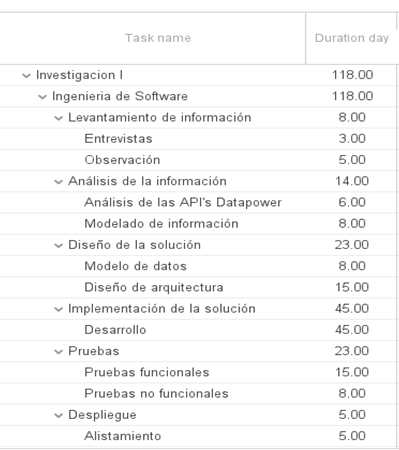
\includegraphics[width=1.0\textwidth]{parte1/img/tareas.png}
%%        \caption{Tareas}
%%    \end{figure}
\subsection*{Diagrama de grantt}

\begin{figure}[th!]
    \begin{ganttchart}[
            vgrid, 
            hgrid,
            y unit chart = .5cm,
            x unit = .6cm
            ]{1}{17}
        \ganttset{bar height=.2}{group height=.4}{group label node/.append style={align=rigth}}
        \gantttitle{Prototipo Administración centralizada DP.}{17} \\
        \gantttitle{SEMANAS}{17} \\
        \gantttitlelist{1,...,17}{1}\\
        \ganttgroup{Levantamiento Información}{1}{2} \\
            \ganttbar{Entrevistas}{1}{1} \\
            \ganttlinkedbar{Observación}{2}{2} \\
        \ganttgroup{Análisis de Información}{2}{3} \\
            \ganttbar{Análisis de las API de DP}{2}{2} \\
            \ganttlinkedbar{Modelado de la información}{3}{3} \\
        \ganttgroup{Diseño de la solución}{4}{7} \\
            \ganttbar{Modelado de datos}{4}{5} \\
            \ganttlinkedbar{Diseño de la arquitectura}{6}{7} \\
        \ganttgroup{Implementación de la solución}{7}{13} \\
            \ganttbar{Desarrollo Fase 1}{7}{11} \\
            \ganttlinkedmilestone{Primero prototipo}{11} \\
            \ganttlinkedbar{Desarrollo Fase 2}{12}{13} \\
        \ganttgroup{Pruebas}{14}{16} \\
            \ganttbar{Pruebas Funcionales}{14}{15} \\
            \ganttlinkedmilestone{Segundo prototipo}{15} \\
            \ganttlinkedbar{Pruebas No Funcionales}{16}{16} \\
        \ganttgroup{Despliegue}{17}{17} \\
            \ganttbar{Alistamiento}{17}{17} \\
    \end{ganttchart}
    \caption{Diagrama de grantt}
\end{figure}